\section{Cross-lingual Word Sense Disambiguation}

Cross-lingual word sense disambiguation (CL-WSD) is the task of labeling words
or phrases in some input sentence with their contextually-appropriate
translations into some target language.
It is a variant of the more general WSD
task, with the sense inventory for each word defined as its possible
translations.
This setting for WSD has an immediate application in machine translation, since
many words have multiple possible translations.

WSD in translation has a long history; practical work in integrating
WSD with statistical machine translation dates back to early SMT work at IBM
\cite{Brown91word-sensedisambiguation}, but the problem itself was described in
Warren Weaver's prescient 1949 memorandum \cite{weavermemo}, which describes a
modern conception of word sense disambiguation.

In the early history of machine translation, researchers were very concerned
with WSD; to some, it seemed an insurmountable problem. As Bar-Hillel wrote,
concerning writing a program to translate sentences like \emph{The box was in
the pen.} \cite{barhillel1960}:

\begin{quote}
... I know of no program that would enable a machine to come up with this
unique rendering unless by a completely arbitrary and ad hoc procedure whose
futility would show itself in the next example.
\end{quote}

To produce a correct rendering of this sentence in Spanish, for example, the
translation system must decide between translating ``pen" as \emph{corral} (an
enclosure, like for an animal) or as \emph{pluma} (the instrument for writing).
As of this writing, for this particular example, Google Translate picks the
less-sensible ``in the writing implement" translation. One wonders how this
could come about -- we would hope that the n-gram language model for Spanish
would prefer sentences about things in enclosures than things in writing
implements, but then the word \emph{en} is a translation of both the English
``in" and ``on", and \emph{pluma} can also mean ``feather". This situation is
fairly complex.

\begin{figure}
  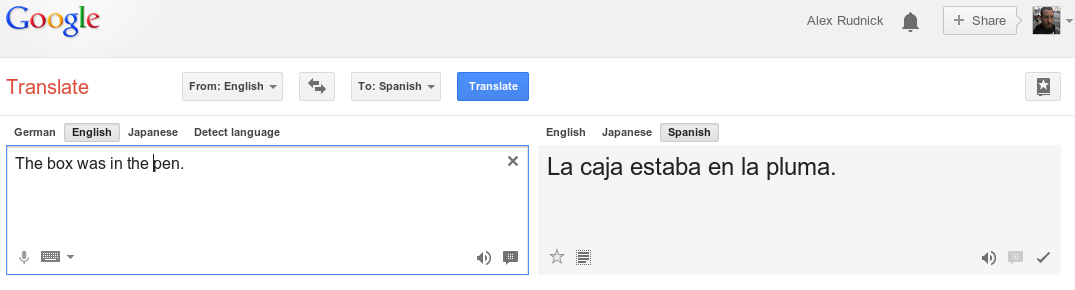
\includegraphics[width=12cm]{box-in-pen.png}
  \caption{Google Translate, September 17, 2013; interestingly, adding or
  removing the final period in the English sentence causes a switch between the
  ``pluma" and ``corral" renderings.}
  \label{fig:box-in-pen}
\end{figure}

In general, there is a many-to-many relationship between words across language
boundaries. Translation is not easy.
%%% OK.

\begin{figure}
  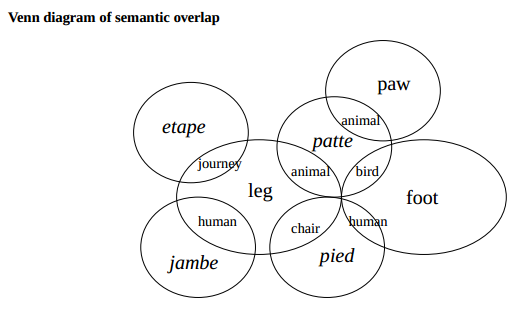
\includegraphics[width=12cm]{hutchins-leg-etc.png}
  \caption{Overlap of words related to ``leg"; relationships between English
  and French words. Figure 21.2 from \protect\cite{slp1}; example originally
  from \protect\cite[Chapter 6]{hutchins1992introduction}.}
  \label{fig:leg}
\end{figure}






This framing has received enough attention to warrant shared tasks at recent
SemEval workshops; the most recent running of the task is described in
\cite{task10}.

Intuitively, machine translation implies an ``all-words" WSD task: we need to
choose a translation for every word or phrase in the source sentence, and the
sequence of translations should make sense taken together.





Despite this, most SMT systems do not use an explicit WSD module
\cite{wsdchap3}, as the language model and phrase tables of these systems
mitigate lexical ambiguities somewhat.


There have been shared tasks on CL-WSD at recent SemEval workshops; the most
recent running of the task is described in \cite{task10}.


We will develop and extend at least two broad approaches for CL-WSD: the use
of multilingual evidence where available and sequence labeling.

Both of these techniques have been prototyped and presented at workshops, but
they will be refined significantly and integrated into a more general tool for
use in practice with MT systems.

\subsection{Using multilingual evidence}
For many languages, we have multiple bitext corpora, where each corpus covers a
different language pair. There are, for example, many bitext corpora available
for English and other languages, or for Spanish and other languages.
We would like to be able to make use of evidence from all of these corpora when
translating into any particular target language, if possible.
Each corpus may contain useful examples of a given source-language word,
and senses of that word may be lexicalized in varying, non-overlapping ways in
the different target languages.
We would want a CL-WSD system to be able to pick up on the relationships
between senses of a given word -- two target languages may happen to surface
the same sense distinctions, perhaps due to being related languages, or simply
by coincidence. Alternatively, a combination of translations into several
languages may provide evidence for a certain lexical choice in the target
language.

We could also imagine using a sense-annotated corpus to train a ``monolingual"
WSD system, and use this as a 
... basically ensemble methods for WSD.

This approach is informed by the work of Lefever and Hoste
\cite{lefever-hoste-decock:2011:ACL-HLT2011}, although their technique requires
an entire machine translation system to perform CL-WSD, which is somewhat
unwieldy when we want to use CL-WSD as a subcomponent of a machine translation
system.

Earlier this year, we developed a prototype CL-WSD system that makes use of
multilingual evidence \cite{rudnick-liu-gasser:2013:SemEval-2013} and produced
some of the best results in a SemEval shared task on CL-WSD \cite{task10}.
The task was to translate polysemous nouns from English into other European
languages. In our SemEval paper, we presented three variations on the approach:
a straightforward classification approach (without multilingual evidence), a
classifier stacking approach, and a graphical model system based on loopy
belief propagation over Markov networks.

The simplest system presented in that work, based on a maximum entropy
classifier, simply extracted features from a window around the English noun to
be translated and used these to make a prediction. The same system could also
return a probability distribution over target-language words or phrases. This
simple system was used as a subcomponent in the two more sophisticated systems.

The classifier stacking approach used 
for each available bitext corpus, for each source-language word that we want to
model, we train a classifier to predict translations from the source language
into the other language of the bitext.
Then we can include the output of that classifier as a feature when training
our classifier for the desired target language.


In the graphical model approach, we treat the problem of 
... this also has the property of explicitly handling the uncertainty of each
of the component classifiers.

\subsection{Lexical selection as a sequence labeling problem}
We will also investigate the use of sequence-labeling models for lexical
selection.  The intuition behind the sequence-labeling approach is that machine
translation implies an ``all-words" WSD task, in that we need to choose a
translation for every word or phrase in the source sentence, and that the
sequence of translations chosen should make sense when taken together.

One promising formalism for this line of work is the Maximum Entropy Markov
Model \cite{icml00/mccallum}, which can be combined in a straightforward way
with the simpler Hidden Markov Model (HMM).
This combination allows for efficient inference and the ability to trade more
computational resources for richer modeling. More sophisticated sequence
models, such as Conditional Random Fields, may be useful in this task as well.

We also developed a prototype CL-WSD system based on sequence labeling and
applied it to both English-Spanish and Spanish-Guarani translation tasks; this
work was presented at the HyTra workshop in August
\cite{rudnick-gasser:2013:HyTra-2013}.

For the sequence labeling approach in which only some words have their
translations modeled explicitly with a classifier, we have yet to explore what
the best approaches are for choosing \emph{which} words should get classifiers.

We will also look into the best ways to integrate the multilingual approach
with this one.

TODO look at the papers Nathan sent and be able to explain what other people
are doing for hard sequence labeling problems. That might go in the related
work section, or perhaps here.

\subsection{CL-WSD system combination}

Think about and expand the conversation I had with Markus.

You could imagine different CL-WSD systems rating each option separately and
then using MERT to get like an ensemble.
The question we were trying to address is like:
what if your n-gram model over labels for your source language has one idea
(this is the next likely label), and your emission probabilities say something
else (this is the label most likely to generate the observed input word)...
well, we could imagine just making several different decisions and letting the
decoder sort it out. We're doing that already actually, by including
phrase-table probabilities and a language model.
Are we just converging on the idea of a log-linear model again?
But the point here is that we don't have to have just one CL-WSD system. We can
have a bunch and let them fight it out. Hopefully this will help!

\subsection{Applying similar techniques for morphology prediction}

Sequence labeling has also been applied to the problem of generating
morphological features in target language text, so that target language output
words are appropriately inflected...
\cite{toutanova-suzuki-ruopp:2008:ACLMain}

This will be one of the approaches we investigate in the development of
Tereré...

